\documentclass{bmvc2k}
\usepackage[ruled]{algorithm2e}
\begin{document}

\section*{digital image processing hw1}
\subsection*{problem 1: piecewise linear transformation}

hw1\_1.m loads cameraman.tif image file, applies two different piecewise 
linear transform to the image, and plot the images in order.

PiecewiseLinearTr.m defines piecewise linear transform of given input and 
output transformed image.
Here is the pseudocode for implementing PiecewiseLinearTr.m.

\begin{algorithm}
\caption{PiecewiseLinearTr.m}
$output \gets zeros$\;
$slope \gets zeros$\;
$y\_inter \gets zeros$\;
\For{$i = 1:(len(a)-1)$}{
    $slope_i \gets (b(i+1) - b(i)) / (a(i+1) - a(i))$\;
    $y\_inter_i \gets (a(i+1) * b(i) - a(i) * b(i+1)) / (a(i+1) - a(i))$\;
}

\For{$i = 1:M$}{
    \For{$j = 1:N$}{
        \For{$k = 1:(len(a)-1)$}{
            \If{$input(i,j)$ between $a(k), a(k+1)$}{
                $output(i,j) = slope_k * input(i,j) + y\_inter_k$\;
            }
        }
    }
}
\end{algorithm}

Result of hw1\_1.m can be found in \figurename{\ref{fig:1}}. The leftmost one is the original image, 
middle is the transformed version with segment coordinates of [0,1], [1,0]. The rightmost one is from the
segment coordinates of [0 .25 .5 .75 1],[0 .75 .25 .5 1].

\begin{figure}[h]
    \centering
    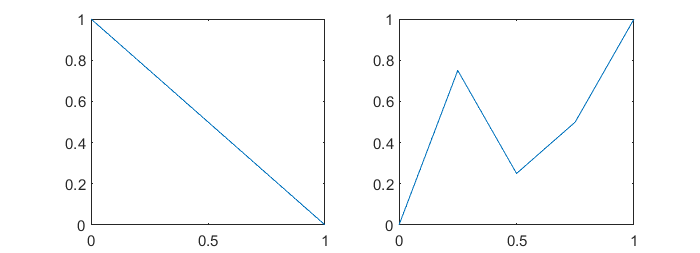
\includegraphics[scale=0.25]{hw1_1_2}
    \caption{transformation functions. 
    left: coordinates of [0,1], [1,0], right: coordinates of [0 .25 .5 .75 1],[0 .75 .25 .5 1].}
    \label{fig:2}
\end{figure}

\figurename{\ref{fig:2}} plots two transformation functions. It can be seen that left transformation
inverses the input intensity, which is proved on middle version of \figurename{\ref{fig:1}}.
In the rightmost cameraman image, darkest part like coat is whitened and background, which has relatively
high intensity, is darkened. This corresponds with right function of \figurename{\ref{fig:2}}.  

\begin{figure}[h]
    \centering
    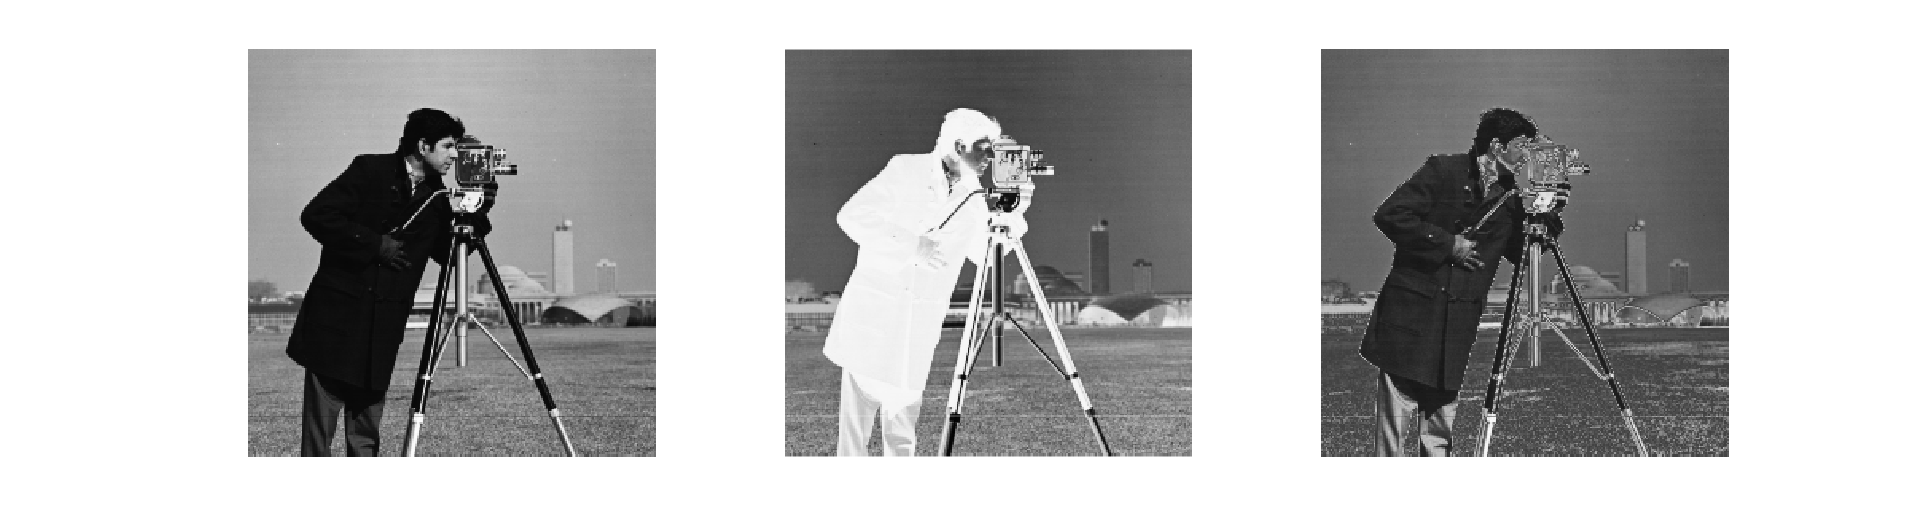
\includegraphics[scale=0.25]{hw1_1}
    \caption{result of running hw1\_1.m}
    \label{fig:1}
\end{figure}

\subsection*{problem 2: image histogram}

hw1\_2.m loads input.jpg and plot histogram of the image.
Hist.m implements gathering histogram statistics.
Below is the pseudocode for the file.

\begin{algorithm}
\caption{Hist.m}
$hist \gets zeros$\;
\For{$i = 1:M$}{
    \For{$j = 1:N$}{
        $hist(input(i,j)) += 1$\;
    }
}
plot $hist$\;
\end{algorithm}

\figurename{\ref{fig:3}} is the result of the hw1\_2.m. 

\begin{figure}[h]
    \centering
    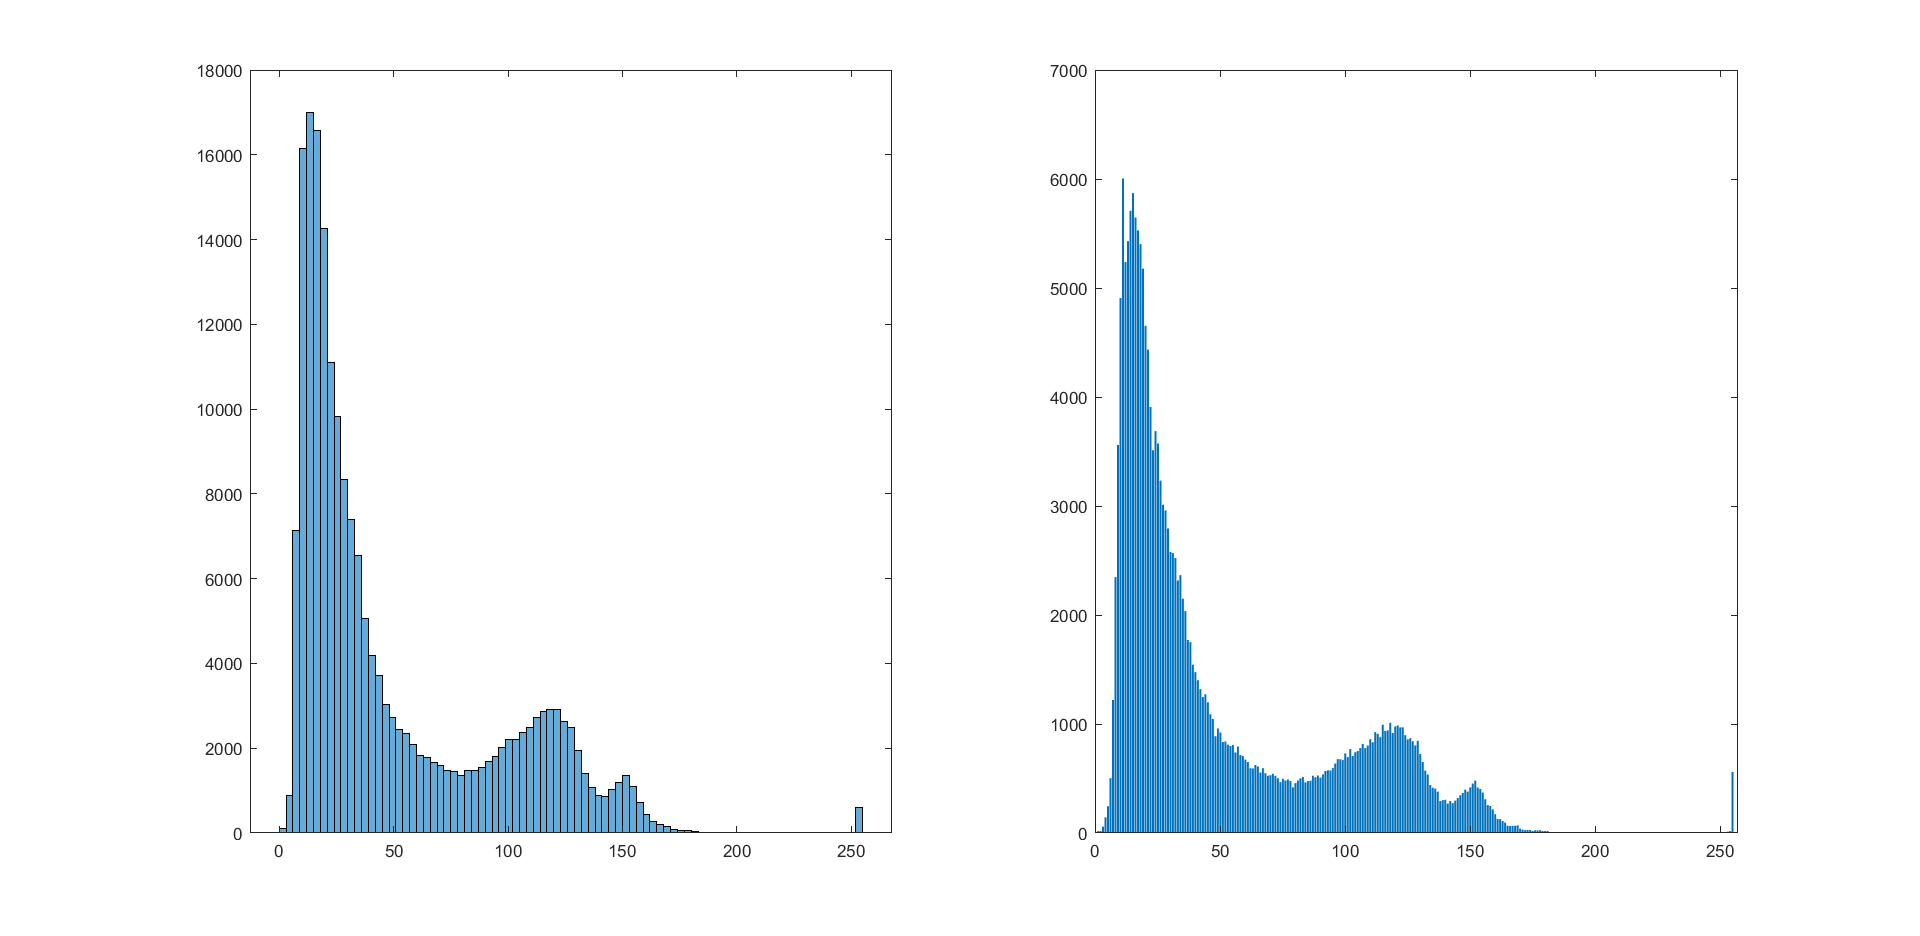
\includegraphics[scale=0.25]{hw1_2}
    \caption{histogram visualizations.}
    \label{fig:3}
\end{figure}

\subsection*{problem 3: histogram equalization}

hw1\_3.m loads input.jpg and applies histogram equalization.
HistEq.m accepts input as image and output histogram-equalized version of the image.
The pseudocode for HistEq.m is as follows.

\begin{algorithm}
\caption{HistEq.m}
$hist \gets zeros$\;
$transform \gets zeros$\;
\For{$i = 1:M$}{
    \For{$j = 1:N$}{
        $hist(input(i,j)) += 1$\;
    }
}
    
\For{$i = 1:L$}{
    $z \gets sum(hist(1:i))$\;
    $z \gets z * (L-1) / (M * N)$\;
    $transform(i) \gets z$\;
}

$output \gets input$\;
\For{$i = 1:M$}{
    \For{$j = 1:N$}{
        $output(i,j) \gets transform(input(i,j))$\;
    }
}
\end{algorithm}

\figurename{\ref{fig:4}} depicts the result. It can be seen that the resulting
image has enhanced contrast. Detailed histogram can be found in \figurename{\ref{fig:5}}.

\begin{figure}[h]
    \centering
    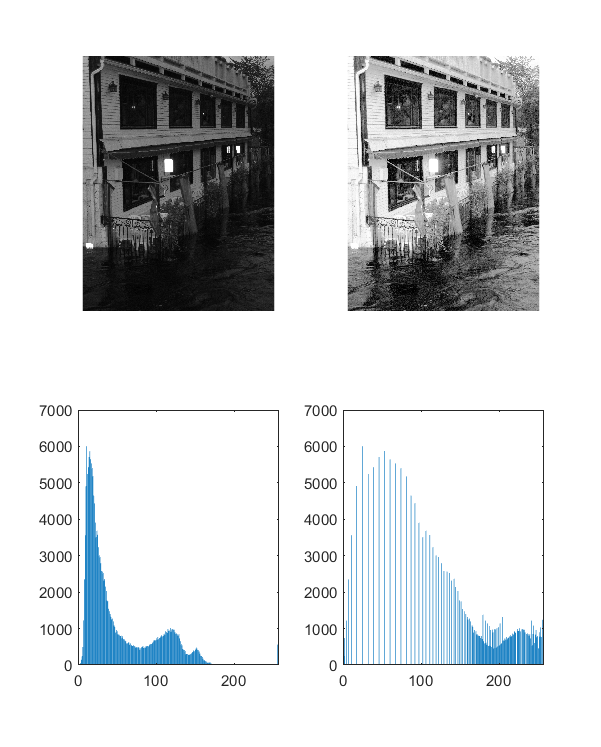
\includegraphics[scale=0.25]{hw1_3}
    \caption{histogram visualizations.}
    \label{fig:4}
\end{figure}

Transformed histogram follows more to uniform than the original.

\begin{figure}[h]
    \centering
    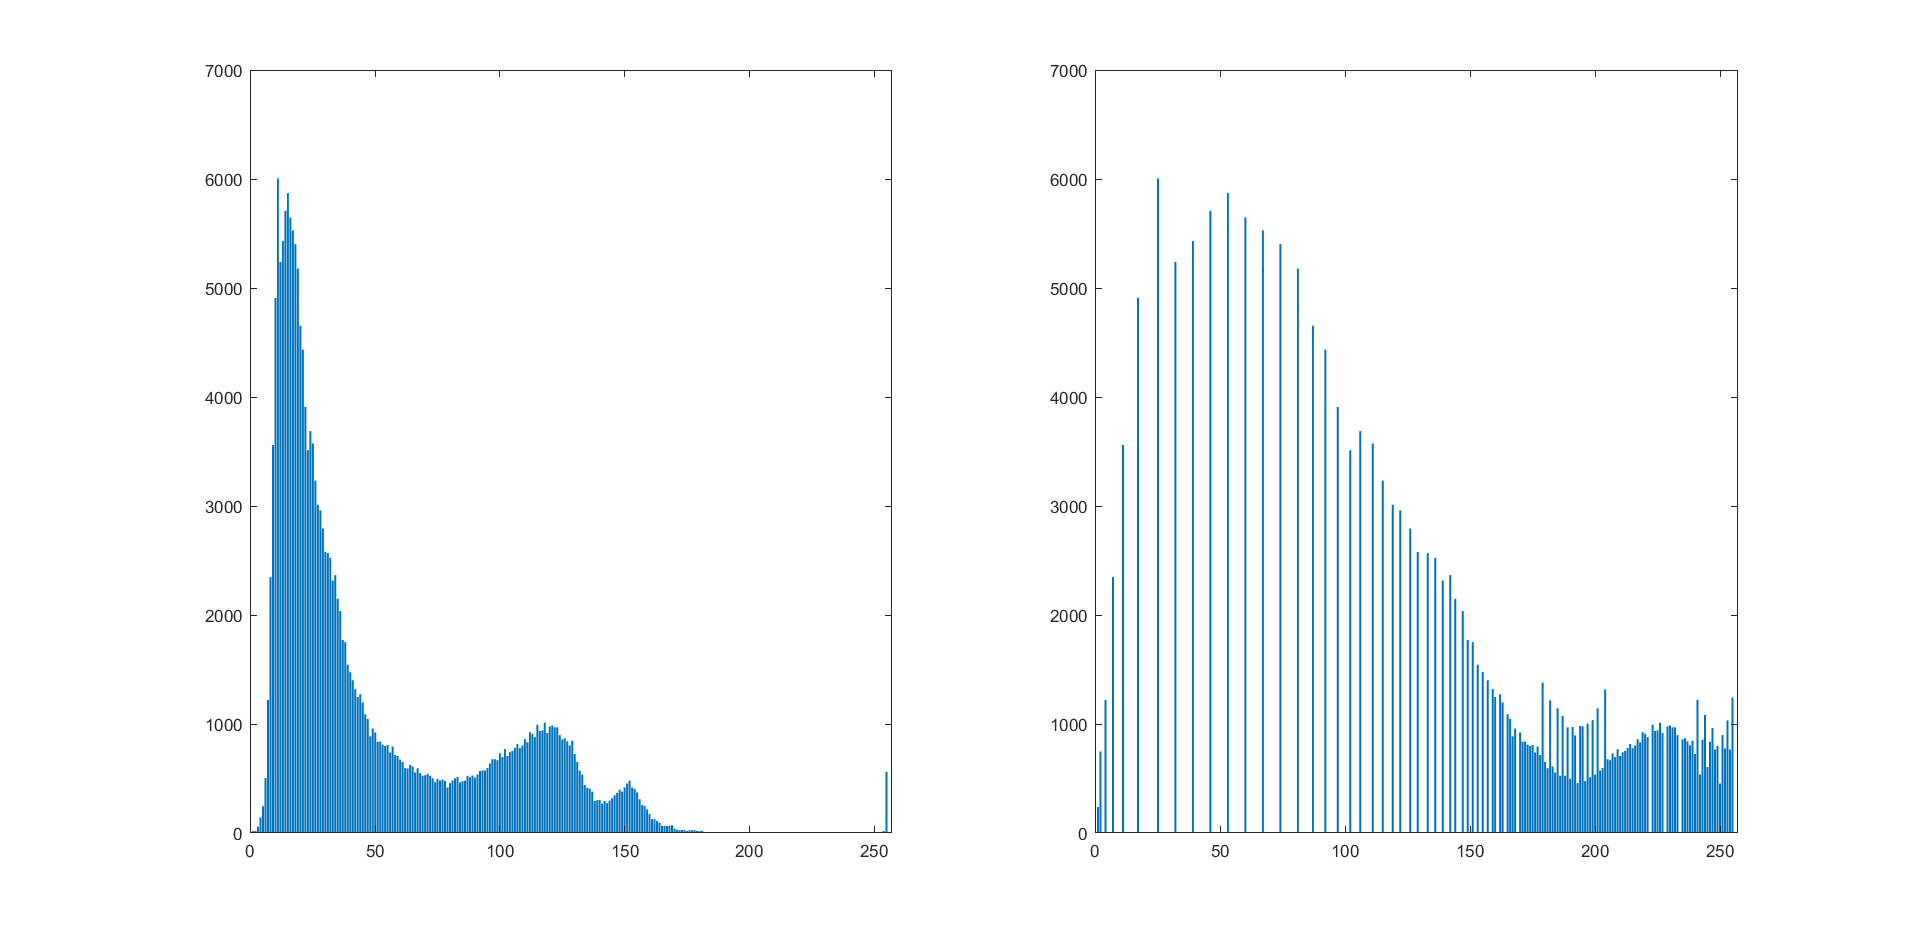
\includegraphics[scale=0.25]{hw1_3_2}
    \caption{histogram visualizations.}
    \label{fig:5}
\end{figure}

\subsection*{problem 4: histogram equalization}

\subsection*{problem 5: histogram matching}

\end{document}
